% easychair.tex,v 3.5 2017/03/15

\documentclass{easychair}
%\documentclass[EPiC]{easychair}
%\documentclass[EPiCempty]{easychair}
%\documentclass[debug]{easychair}
%\documentclass[verbose]{easychair}
%\documentclass[notimes]{easychair}
%\documentclass[withtimes]{easychair}
%\documentclass[a4paper]{easychair}
%\documentclass[letterpaper]{easychair}

\usepackage{doc}
\usepackage{tikz}
\usepackage{tikzsymbols}
\usepackage{pifont}
\newtheorem{theorem}{Theorem}
\usetikzlibrary{arrows}

%\usepackage[firstpageonly=false, color={[gray]{0.5}},
%   scale=2.0, text=DRAFT]{draftwatermark}
% -------------------------------
%%%% For Alectryon

\usepackage{texments}
%%% for movies by alectryon
\usepackage{../movies/snippets/assets/alectryon}
\usepackage{../movies/snippets/assets/pygments}
%%% One hypothesis per line 
\makeatletter
\renewcommand{\alectryon@hyps@sep}{\alectryon@nl}
\makeatother

%%% \snippets{A,B,C,…} inputs a series of snippets as one block (with \itemsep
%%% between them).  A, B, C should be paths to files in movies/snippets/.
\usepackage{etoolbox}
\makeatletter
\newcommand{\inputsnippets}[1]
  {{\setlength{\itemsep}{1pt}\setlength{\parsep}{0pt}% Adjust spacing
    \alectryon@copymacros\begin{io}
      \forcsvlist{\item\@inputsnippet}{#1}
    \end{io}}}
\let\input@old\input % Save definition of \input
\newcommand{\@inputsnippet}[1]
  {{\renewenvironment{alectryon}{}{}% Skip \begin{alectryon} included in snippet
    \input@old{#1}}}
\makeatother

%---------------------------- 
\newcommand{\canonseq}[2]{\mbox{$\{#1\}(#2)$}}

\usepackage{varioref}
\newtheorem{todo}{To do}
\usepackage{amsfonts, afterpage}

\newcommand{\easychair}{\textsf{easychair}}
\newcommand{\miktex}{MiK{\TeX}}
\newcommand{\texniccenter}{{\TeX}nicCenter}
\newcommand{\makefile}{\texttt{Makefile}}
\newcommand{\latexeditor}{LEd}


%\makeindex

%% Front Matter
%%
% Regular title as in the article class.
%
\title{Hydras, Ordinals \&  Co.  \\
  A library in Coq of entertaining formal mathematics}



\author{
Pierre Castéran \inst{1}
\and
    Jérémy Damour \inst{2}
\and
Karl Palmskog \inst{3}
\and Clément Pit-Claudel \inst{4}
\and Théo Zimmermann \inst{5}
}


\institute{
Univ. Bordeaux, CNRS, Bordeaux INP, LaBRI, UMR 5800, F-33400 Talence, France \\
  \email{pierre.casteran@labri.fr}
\and
Univ. de Paris, F-75013 Paris, France
\and
KTH Royal Institute of Technology, Stockholm, Sweden
\and
MIT CSAIL, Cambridge, Massachusetts, USA
\and
Inria, Univ. de Paris, CNRS, IRIF, UMR 8243, F-75013 Paris, France
}



\authorrunning{Castéran, Damour, Palmskog, Pit-Claudel and Zimmermann}

\titlerunning{Hydras, Ordinals \& Co.}

\newcommand{\TODO}[2][]{[\textcolor{red}{TODO (#1):} \emph{#2}]}

\begin{document}

\maketitle


\begin{abstract}
  \emph{Hydra-battles} is a collaborative library on discrete math, written for the Coq proof assistant, and developed under the \emph{Coq-community} project. The proof scripts are
  accompanied with an electronic book, made with the help of the \emph{Alectryon} litterate proving tool.
  We present the evolution of the mathematical contents since
  former presentations at JFLA meetings.
  Then, we show how the structure of the project is determined   by two  requirements which must continuously satisfied:
   maintenance of the library with respect to several Coq-community projects it requires and evolutions of Coq, and 
  consistency of the book with respect to the library. 
\end{abstract}


% \setcounter{tocdepth}{2}
% {\small
% \tableofcontents}


%------------------------------------------------------------------------------
\section{Introduction}
\label{sect:introduction}

\subsection{Background}

\begin{itemize}
\item formalizations of mathematics in proof assistants, such as Coq, continually grow in size and scope
\begin{itemize}
\item the Mathematical Components library and the four-color theorem and the odd order theorem in Coq
\item the Mathlib library for Lean
\end{itemize}
\item to continue to be useful as examples and reusable libraries, formalizations must be well \emph{documented} and \emph{maintained} to ensure they work with new proof assistant releases \TODO[Pierre]{add evolution of styles of proof and formalization (not limited to Coq litterature)? } 
\item Lean and Mathematical Components have accompanying books, which are written mainly to onboard new library users
\item book authors faced with several design choices: literate documents, using tools to keep the book and the proof assistant synchronized
\end{itemize}

\subsection{Vision}
The \emph{Hydra-battles} project, part of \emph{Coq-community}~\cite{CoqCommunity} aims to be an experimental platform for the collaborative development of commented libraries of formal proofs. \emph{Coq-community} is a community organization that we have founded in 2018 with two goals in mind: providing a solution for the long-term maintenance of interesting Coq packages, and working collaboratively on documentation projects. The \emph{Hydra-battles} project demonstrates that these two goals are not independent: interesting Coq packages can become the basis for new documentation.
%
This umbrella project now includes evolved versions of the former Cantor and Additions libraries (under the new names of Hydra-battles and Addition-chains), the Pocklington library, extracted from Russel O'Connor's Goedel library~\cite{OConnor05, Goedel} and a bridge to the Gaia library (by José Grimm~\cite{Gaia,grimm:hal-00911710}).
%
By following this approach of commenting interesting Coq packages, we provide new documentation content, that contributes to the diversity of the thriving Coq documentation ecosystem.

We call on the Coq users in the JFLA community and beyond to come and join us in this effort, by bringing new interesting projects which are worth presenting to Coq learners, \emph{a.k.a.} Coq users, and guiding them in their exploration.
%
We also always have project ideas to extend further our explorations and anyone is welcome to join the team by sending small or larger contributions through pull requests.
%
The current state of the project is already the result of such evolutions after several of us contributed project solutions and new proposals to the initial version of the first author.

Futhermore, contrary to traditionally published books, the ``book'' that forms part of this project is intended to be forever evolving. As new Coq formalization patterns and proof techniques appear, the book can be adapted to demonstrate their use (in case they fit well with our applications).
%
By using modern maintenance techniques such as continuous integration and deployment, we can ensure that this documentation stays up to date with the latest Coq releases. With Alectryon~\cite{alectryonpaper, alectryongithub}, we ensure that code and documentation are always in sync.

\subsection{Hydra games}
Hydra games (also known as \emph{Hydra battles}) appear in an article published in 1982 by two mathematicians, 
Laurie Kirby and Jeff Paris: \emph{Accessible Independence Results for Peano Arithmetic}~\cite{KP82}.
This article describes a game between two players: Hercules and a hydra.
A short description of the game  can be found in~\cite{bauer2008, KP82, JFLA2018paper}. One can also play with
Andrej Bauer's simulator~\cite{BauerHydra}.
In a few words:
\begin{itemize}
\item A hydra is a finite tree, traditionally presented with the root at the bottom, the leaves of which are called \emph{heads}
  (Fig~\ref{fig:round}).
\item At every round, Hercules chops off one head of the hydra. If the head is at a distance greater than 1 from the root,
  then some sub-tree $h$ of the hydra is copied a certain amount $n$ of times. The number $n$ of copies and the sub-tree $h$ may depend of the considered variant of the game
  or the time elapsed since the beginning of the fight.
  Figure~\ref{fig:round} shows an example with $n=2$.
\end{itemize}



\begin{figure}[h]
  \centering
  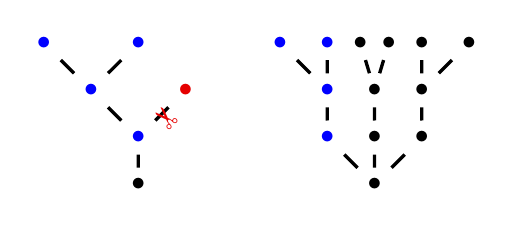
\begin{tikzpicture}[very thick, scale=0.3]
  \node (h1) at (4,0){$\bullet$};
  \node[blue] (h2) at (4,2){$\bullet$};
  \node[blue] (h3) at (2,4){$\bullet$};
  \node[blue] (h4) at (0,6){$\bullet$};
  \node[blue] (h5) at (4,6){$\bullet$};
  \node[red!90!black] (h6) at (6,4){$\bullet$};
  \draw (h1) -- (h2) ;
  \draw (h2) -- (h3) ;
  \draw (h2) -- node[red!90!black,font=\small,sloped,shift={(0.01,-0.075)},rotate=90]{\textbf{\ding{34}}} (h6);
  \draw (h3) -- (h4) ;
  \draw (h3) -- (h5) ;
 
\node (hn1) at (14,0){$\bullet$};
\node[blue] (hn2) at (12,2) {$\bullet$};
\node[blue] (hn3) at (12,4) {$\bullet$};
\node[blue] (hn4) at (10,6){$\bullet$};
  \node[blue] (hn5) at (12,6){$\bullet$};
  \draw (hn1) -- (hn2) ;
  \draw (hn2) -- (hn3) ;
  \draw (hn3) -- (hn4) ;
  \draw (hn3) -- (hn5) ;
\node (hn2b) at (14,2) {$\bullet$};
\node (hn3b) at (14,4) {$\bullet$};
\node (hn4b) at (13.4,6){$\bullet$};
  \node (hn5b) at (14.6,6){$\bullet$};
  \draw (hn1) -- (hn2b) ;
  \draw (hn2b) -- (hn3b) ;
  \draw (hn3b) -- (hn4b) ;
  \draw (hn3b) -- (hn5b) ;
  \node (hn2c) at (16,2) {$\bullet$};
\node (hn3c) at (16,4) {$\bullet$};
\node (hn4c) at (16,6){$\bullet$};
  \node (hn5c) at (18,6){$\bullet$};
  \draw (hn1) -- (hn2c) ;
  \draw (hn2c) -- (hn3c) ;
  \draw (hn3c) -- (hn4c) ;
  \draw (hn3c) -- (hn5c) ;
\end{tikzpicture}

  \caption{Two successive states of a hydra in a battle.  Hercules chopped off the rightmost head of the hydra (red), and the whole left tree except the root node (blue) was copied twice.}
  \label{fig:round}
\end{figure}



 %  \begin{figure}[htb]
% \centering
% \begin{tikzpicture}[very thick, scale=0.3]
% \node (foot) at (10,0) {$\bullet$};
% \node (N1) at (2,2) {$\bullet$};
% \node (N2) at (10,2) {$\bullet$};
% \node (N22) at (7,2) {$\bullet$};
% \node (N3) at (14,2) {$\bullet$};
% \node (N4) at (18,2) {$\Smiley[2][green]$};
% \node (N5) at (0,4) {$\bullet$};
% \node (N6) at (2,5) {$\Smiley[2][green]$};
% \node (N7) at (4,6) {$\Smiley[2][green]$};
% \node (N88) at (7,4) {$\bullet$};
% \node (N8) at (10,4) {$\bullet$};
% \node (N9) at (14,6) {$\Smiley[2][green]$};
% \node (N10) at (0,8) {$\Smiley[2][green]$};
% \node (N11) at (10,7) {$\Smiley[2][green]$};
% \node (N111) at (7,7) {$\Smiley[2][green]$};
% \draw (foot) to [bend left=10] (N1);
% \draw (foot) -- (N2);
% \draw (foot) -- (N22);
% \draw (foot) -- (N3);
% \draw (foot) -- (N4);
% \draw (N1) to  (N5);
% \draw (N1) to   [bend left=10] (N6);
% \draw (N1) to   [bend right=20] (N7);
% \draw (N2) to  (N8);
% \draw (N22) to  (N88);
% \draw (N8) to  (N11);
% \draw (N88) to  (N111);
% \draw (N3) to  (N9);
% \draw (N5) to  (N10);
% \end{tikzpicture}
% \caption{The hydra associated with the ordinal $\omega^{\omega+2}+\omega^\omega \times 2 + \omega + 1$ \label{fig:iota-example}}

% \end{figure}

Kirby and Paris prove the following theorems, applying
combinatorial results about ordinal numbers by Jussi Ketonen and Robert Solovay~\cite{KS81}.

\begin{theorem}
  In the Hydra game, Hercules eventually wins, whichever the strategy of both players :
  choice of a head to chop off, choice of the number of copies. 
 \label{kp:thm1}
\end{theorem}

\begin{theorem}
  Theorem~\ref{kp:thm1} cannot be proved in Peano Arithmetic. \label{kp:thm2}
\end{theorem}

The contrast between the simplicity of the statements above and the complexity of their proofs convinced us that it is a good theme for a commented library~\cite{HydraBattles} of formal proofs written for the \textit{Coq} proof assistant~\cite{Coq}. 

Complex formalisations and proofs are explained in an
  electronic book~\cite{HydraBook} (PDF document of over 280 pages). Whenever various reasonable choices exist, we try to present and compare the alternatives.
  For instance, Figures~\ref{fig:Ex42E0} and \ref{fig:Ex42-schutte} show two radically different proofs of the equality
  $\omega+42+\omega^2=\omega^2$. The first one is a simple proof by computation, the second one shows how this equality
  is a consequence of the axioms of the set-theoretic model  by Kurt Schütte~\cite{schutte}. 

This work is also an opportunity to 
 provide ``concrete'' examples of formalization and proof techniques: operational type classes, functions defined by  equations, dependently typed functions, etc. It may be also used as a library on ordinal numbers, for instance for proving termination properties.

 Prior stages of this project have already been presented at
 JFLA~\cite{PCiota, JFLA2018paper}.
We present recent evolutions of the library: new results, interaction within the Coq-community project~\cite{CoqCommunity}, and documentation generated with Alectryon~\cite{alectryonpaper, alectryongithub}.

\section{Changes in the library}
The 2018 article~\cite{JFLA2018paper} contains a formal proof of  a variant of Theorem~\ref{kp:thm2}:

\begin{theorem}
  Let $\mu$ be any ordinal strictly less than $\epsilon_0$.
  There is no function mapping hydras to the segment $[0,\mu)$, which could be used as a measure for  proving the termination of  all hydra battles.\label{thm3}
\end{theorem}

\TODO[Clément]{Is there a word missing above?}
Considering measures applicable to \emph{all} battles allowed us to
focus on battles where the hydra can make an arbitrary number of copies at any time, which made our proof by contradiction artificially easier.
Unfortunately, the examples  most commonly shown in the litterature
(see for instance~\cite{KP82, bauer2008, BauerHydra}) 
assume that the hydra grows $n$ copies at step $n$ of the game, which is incompatible with our proof.

\vspace{6pt}

We prove now that Theorem~\ref{thm3} still holds with these typical battles by borrowing new combinatorial results from~\cite{KS81}.
Without loss of generality, we assume the following restrictions:
 
 \begin{itemize}
   \item The game starts at an initial step $i\in\mathbb{N}$ (not necessarily $0$).
   \item  The hydra is always the  representation as a tree of some ordinal strictly below $\epsilon_0$ in Cantor normal
     form. For instance, Fig~\ref{fig:round} shows the hydras respectively associated with  $\omega^{\omega^2+1}$ and $\omega^{\omega^2}\times 3$.
 
 \item Hercules always chops off the rightmost head of the hydra.
 \end{itemize}
 
 In mathematical terms, if at step $n$ the hydra is associated with the ordinal $\alpha$, at step $n+1$ it is associated with
 $\canonseq{\alpha}{n+1}$, the $(n+1)$th element of the canonical sequence of $\alpha$~\cite{KS81}.

 Our new proof of Theorem~\ref{thm3} is based on a systematic study of strictly decreasing sequences of ordinals below $\epsilon_0$, borrowed from~\cite{KS81}.
 
We also study the number of steps of a battle:
Let $\alpha<\epsilon_0$ be an ordinal. 
We prove that  the number of steps of the battle starting with
$\alpha$ at step $i$ is greater or equal than
$H'_\alpha(i)-i$, where $H'$ is a slight variant of the Hardy hierarchy of rapidly growing functions~\cite{BW85, KS81, Promel2013, Wainer1970}.  The function $H'_\alpha$ is defined by transfinite recursion over $\alpha$ on Figures~\ref{fig:hardy-math}
and~\ref{fig:Hprime}.


\begin{figure}[h]
\begin{align}
  H'_0(i) & = i\\
  H'_\alpha(i) &= H'_{(\canonseq{\alpha}{i+1})}(i)  \quad\textit{if $\alpha$ is a limit ordinal}\\
  H'_{\alpha}(i) &=H'_\beta(i+1) \quad\textit{if $\alpha=\beta+1$}
\end{align}  
  \caption{The $H'$ rapidly growing hierarchy of arithmetical functions}
  \label{fig:hardy-math}
\end{figure}


 \begin{figure}[h]
 \inputsnippets{HprimeDef}
\caption{$H'$ definition with the \texttt{coq-equations}
 plug-in~\cite{sozeau:hal-01671777}}
\label{fig:Hprime}
\end{figure}


Using $H'$s equations as rewrite rules, we can study a realistic example. We take the hydra of figure~\ref{fig:start} and $i=0$ as initial configuration. 
By a sequence of rewritings and inductions, we prove that the number of steps of the considered battle is greater or equal than $2^{2^N}$, where $N=2^{70}-1$.

\begin{figure}[h]
  \centering
  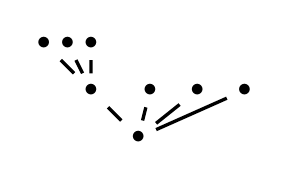
\begin{tikzpicture}[very thick, scale=0.3]
  \node (h1) at (4,0){$\bullet$};
  \node (h2) at (2,2){$\bullet$};
  \node (h3) at (0,4){$\bullet$};
  \node (h4) at (1,4){$\bullet$};
  \node (h5) at (2,4){$\bullet$};
  \node (h6) at (4.5,2){$\bullet$};
  \node (h7) at (6.5,2){$\bullet$};
  \node (h8) at (8.5,2){$\bullet$};
    \draw (h1) -- (h2) ;
    \draw (h2) -- (h3) ;
    \draw (h2) -- (h4) ;
    \draw (h2) -- (h5) ;
    \draw (h1) -- (h6) ;
    \draw (h1) -- (h7) ;
    \draw (h1) -- (h8);
 \end{tikzpicture}

  \caption{The hydra associated with the ordinal $\omega^3+3$}
  \label{fig:start}
\end{figure}




\label{sect:not-pr}

\TODO[Clément]{Highlight `Equations' and remove `omega' highlighting; change theme to something less garish}


More generally, we prove that, for $\alpha\geq\omega^\omega$
the function computing the length of the battle starting with the configuration $(\alpha,i)$ is not primitive recursive.


\section{Integration within Coq-community}





\subsection{Presentation}

\emph{Coq-community} is an informal organization run by volunteer Coq users with objectives to maintain interesting Coq projects in the long-term and help Coq users to collaborate on documentation, tooling, etc.

It was created in 2018, inspired by the \emph{Elm Community} organization~\cite{zimmermann:tel-02451322}.
%
Such ``Community Package Maintenance Organizations'' actually exist in many ecosystems as they avoid the very common problem of an important package becoming unmaintained as its author has moved on or disappeared~\cite{zimmermann2021grounded}.

In the case of Coq, this problem may be even more prevalent as many packages are created by PhD students, or by researchers for a specific paper, but their authors do not intend to maintain the package in the long-term.
%
The authors are however generally very open to having someone else who expresses interest in their work continue the maintenance.
%
\emph{Coq-community} makes that easy by providing a process for transferring or forking an unmaintained package, tooling for setting up good maintenance practices (such as continuous integration) and by making it possible for someone to take over a package without committing in the long-term (as maintainers who drop out can easily be replaced by some other volunteers).
%
Today, \emph{Coq-community} hosts over 50 projects maintained by over 30 maintainers.

\subsection{Interactions with other Coq-community projects}

In order to prove formally that the length of the considered
kind of battles is not given by a primitive recursive function, we used the formalization of primitive recursive functions, part
of Russell O'Connor's contribution on G\"{o}del first incompleteness theorem~\cite{OConnor05, Goedel}.
For this purpose, and above all by consideration of the scientific interest of this contribution, we chose to host and maintain this work within \textit{Coq-community}.

Computability is a key topic in Computer Science teaching. Moreover O'Connor's library is a nice illustration of dependently typed programming, so we chose to devote a full chapter to this formalization, with comments on the definitions and proofs, [counter]-examples and exercises.

% We could already talk a bit of the monorepo structure here, and
% defer some explanations on the tooling to the next section.

\section{Modernizing the infrastructure}
\subsection{Documentation with Alectryon}
\begin{todo}
  Interest of Alectryon:
  \begin{itemize}
  \item Despite the frequent changes (improvements) in the Coq scripts, code inclusion and \textit{Coq}'s answers are up to date.
  \item \TODO[Clément]{A good part of the LaTeX support in Alectryon was developed for hydra-battles, and this was the first real application with a custom driver, too.}
  \item \TODO[Clément]{If you kept a trace of them, I would love to see a discussion of any errors that were caught by including the output systematically instead of copy-pasting it.}
  \item \TODO[Pierre]{the order of appearance of snippets in the book is independent from the module structure}
   \item \TODO[Pierre]{Slicing our proofs into snippets allowed to show only the main parts of our proofsleaved with text (Figure~\ref{fig:Ex42-schutte}).} 
      
  \end{itemize}

   Figures~\ref{fig:Hprime} (code snippet), \ref{fig:Ex42E0} and \ref{fig:Ex42-schutte} have been generated with Alectryon.
\end{todo}


  \begin{figure}[h]
    \centering
    \fbox{
      \begin{minipage}[h]{1.0\linewidth}
        \inputsnippets{Ex42}
      \end{minipage}}
    \caption{A simple proof by computation}
    \label{fig:Ex42E0}
  \end{figure}



%\afterpage{\clearpage}

\begin{figure}[th]
  \centering
  
  

\fbox{\begin{minipage}[h]{1.0\linewidth}
  Let us prove again the equality $\omega+42+\omega^2= \omega^2$. Let us recall that $\omega^2$ is an abbreviation of $\phi_0(2)$,
\emph{i.e} the third  additive principal ordinal.

\inputsnippets{Ex42a} 


Our proof is very different from the computational proof of
Figure~\ref{fig:Ex42E0}.
By definition of additive principal ordinals, 
it suffices to prove the inequality $\omega+42< \phi_0(2)$.

\inputsnippets{Ex42b}

Since the set \textit{AP} of additive principals  is closed under addition
(by Lemma \textit{AP\_plus\_closed}), it suffices to prove the inequalities $\omega<\phi_0(2)$ and $42<\phi_0(2)$.

\inputsnippets{Ex42d, Ex42c, Ex42e}

\end{minipage}
}
\caption{A proof interleaved with text (from the book)}
  \label{fig:Ex42-schutte}
\end{figure}

\subsection{Continuous integration and deployment, opam packaging, etc.}
\section{Conclusion and perspectives}


\TODO{General Conclusion}



%\subsection{Perspectives}

\subsection{Further extensions}

We plan to extend our libraries in two main directions.
The Gaia project~\cite{Gaia}, also maintained on \textit{Coq-community} contains a development by José Grimm~\cite{grimm:hal-00911710}. This library is dedicated  to the implementation in \textit{Coq (SSreflect)} of books from  Bourbaki's Elements of Mathematics. It contains data structures which are compatible with our ordinal notations. 
Our plan is to build a  bridge between  the combinatorial results of \textit{hydra-battles} and the set-theoretic content of \textit{Gaia}, and make possible the transfer of theorems between both libraries.
Another direction would be to write in \textit{Coq} a formal proof of the original statement of Theorem~\ref{kp:thm2}, using O'Connor's formalization of Peano Arithmetic~\cite{Goedel}.

 \emph{Hydra-battles} is not limited to the study of ordinal numbers and applications.
 For instance, we are also developing 
a module about efficient exponentiation algorithms, and hope
to extend our project to new topics.

%\section{Acknowledgments}
%\label{sect:acks}



\label{sect:bib}
\bibliographystyle{plain}
%\bibliographystyle{alpha}
%\bibliographystyle{unsrt}
%\bibliographystyle{abbrv}
\bibliography{../thebib}


\end{document}

